% !TEX root =../LibroTipoETSI.tex
\chapter{PF\_RING}\LABCHAP{PFRING}
\pagestyle{esitscCD}

\epigraph{In almost every computation a great variety of arrangements for the succession of the processes is possible, 
and various considerations must influence the selections amongst them for the purposes of a calculating engine. One 
essential object is to choose that arrangement which shall tend to reduce to a minimum the time necessary for completing 
the calculation.}{Ada Lovelace}

%\lettrine[lraise=0.7, lines=1, loversize=-0.25]{E}{l} 
\lettrine[lraise=-0.1, lines=2, loversize=0.25]{E}n un sistema de monitorización de tráfico, la captura de paquetes es 
un proceso vital. Si se quiere capturar tráfico a una velocidad aceptable, superiores a 1Gbps, es necesario que todo el 
proceso de captura de paquetes esté bien diseñado y sea eficiente. De no serlo, enseguida comenzaremos a notar 
pérdidas de paquetes, y nuestra monitorización no será efectiva.

%TODO unir con lo demás
Ya hemos cubierto la eficiencia en términos de procesamiento de paquetes en los anteriores capítulos. 

\gls{PFRING} es, según su autor Luca Deri, una tecnología que persigue capturar tráfico a $10G$ sin necesitar tarjetas 
especializadas, sin pérdidas y bajo cualquier circunstancia del tráfico, de forma que sea posible crear sondas de 
tráfico software con el mismo rendimiento que las basadas en hardware \cite{LucaDeriPFRING}.

A lo largo de este capítulo, %TODO

\section{Proceso de paquetes por el núcleo linux}\LABSEC{sec:ProcesoPaquetesLinux}
El paso de paquetes a través del núcleo Linux puede ser un importante cuello de botella. %TODO ampliar

\subsection{Reserva de memoria para almacenar el paquete}
El primer paso en la recepción de paquetes es que éste llegue a la tarjeta de red a través de la interfaz física. Tan 
pronto como esto ocurre, y la memoria interna de la \gls{NIC} contiene el paquete completo, ésta es responsable de 
de crear una estructura de datos para almacenar el paquete en la memoria principal del sistema, y copiarlo ahí.

Esta reserva ya incluye un corte en términos de tiempo, ya que dos procesos no pueden reservar memoria al mismo tiempo. 
El sistema tiene una tabla de memoria en la que están anotados los distintos bloques que cada proceso (incluído el 
núcleo) tiene reservada. Si dos procesos reservasen al mismo tiempo, podría ocurrir que reservasen segmentos de memoria 
solapados.

Por tanto, la reserva debe ser sincronizada, y esta sincronización consume un tiempo importante. Tras ello, la copia es 
en modo \gls{DMA}, por lo que la tarjeta obtiene acceso exclusivo a esa memoria y no es necesario la intervención de la 
CPU para copiar los datos.

El paquete es entonces copiado en una estructura de datos \texttt{sk\_buff}. Dicha estructura es bastante grande, y 
puede ir creciendo a medida que lo necesita. Esto incrementa la fragmentación de memoria, ya que al crecer es posible 
que no quepa en su segmento de memoria, y deba moverse a otro segmento mayor.

Por último, existen bastantes datos de la estructura que son privados, y no deben viajar de una capa a otra en el paso 
de información. Por tanto, hay que clonar la estructura al transmitir información\footnote{Si bien hay partes de la 
misma que pueden mantenerse}, lo que redunda en más reservas y más retrasos por sincronía
\cite{skBuffLinuxFoundation}.

\subsection{Notificación del nuevo paquete}
Cuando el paquete al completo es copiado en la memoria principal, es necesario un mecanismo de notificación al 
\gls{controlador}\index{Controlador de Dispositivo} de red de Linux para que éste pueda procesarlo. Se usa, entonces, 
una interrupción hardware.

La interrupción provoca que el núcleo deje de realizar las tareas que esté haciendo para hacer caso a la llegada del 
paquete. Sin embargo, si tenemos demasiados paquetes por segundo, no dejamos a Linux avanzar, y destrozamos la 
planificación de tareas. Este hecho es conocido como Tormenta de Interrupciones\index{Tormenta de Interrupciones} o 
\emph{interrupt storm} \cite{p206}.

En cada interrupción, la función llamada es \texttt{netif\_rx} o \texttt{netif\_receive\_skb}.

\subsubsection{NAPI}
Para evitar la tormenta de interrupciones, se pueden utilizar técnicas como la llamada \emph{device polling}. El 
funcionamiento es el siguiente \cite{beyondDevicePolling}.
\begin{itemize}
 \item Cuando un nuevo paquete llega, la tarjeta genera una interrupción.
 \item El \gls{SO} la maneja de la siguiente forma:
 \begin{enumerate}
  \item Prohíbe (enmascara) futuras interrupciones del dispositivo.
  \item Programa una tarea para atender a la tajeta en un futuro.
  \item Cuando la atiende, levanta la prohibición de interrupciones.
 \end{enumerate}
\end{itemize}

La implementación de esta técnica en Linux es conocida como \gls{NAPI}.

Podemos ver en las figuras \FIG{InterrupcionesNIC} y \FIG{DevicePolling} las diferencias entre un canal saturado 
con un método y otro. Se observa como, en la primera figura, al núcleo no le da tiempo a procesar todos los paquetes 
del canal saturado, y sólo puede procesar una de cada dos. Sin embargo, en la segunda figura, Linux procesa los 
paquetes cuando puede, en tiempos aleatorios, y coge de una tacada todos los paquetes que necesita.

\begin{figure}[hbtp]
\centering
%\hfill
\subfloat[Interrupción]%
   {\LABFIG{InterrupcionesNIC}%
   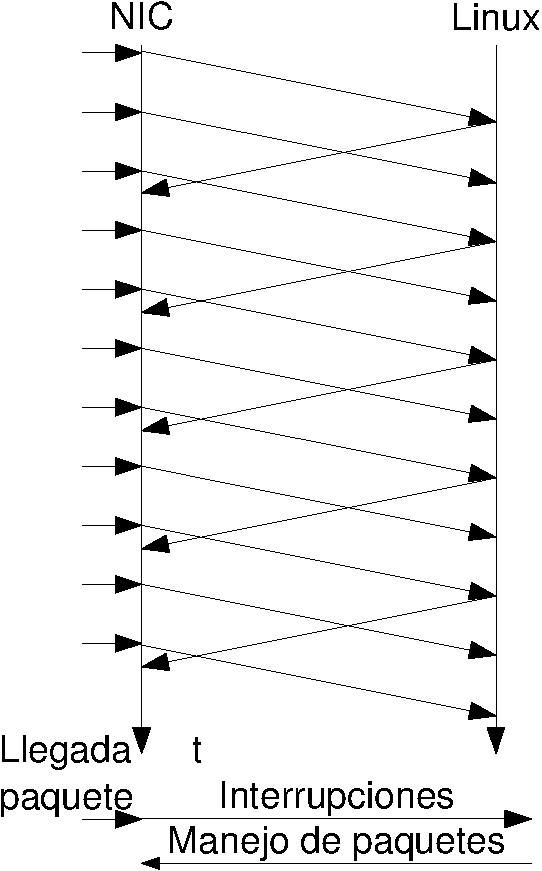
\includegraphics[width=0.30\textwidth]{CapituloPF_RING/Figuras/InterrupcionesNIC-crop}}%
\hspace{0.2\textwidth}
\subfloat[Device Polling]%
 {\LABFIG{DevicePolling}%
 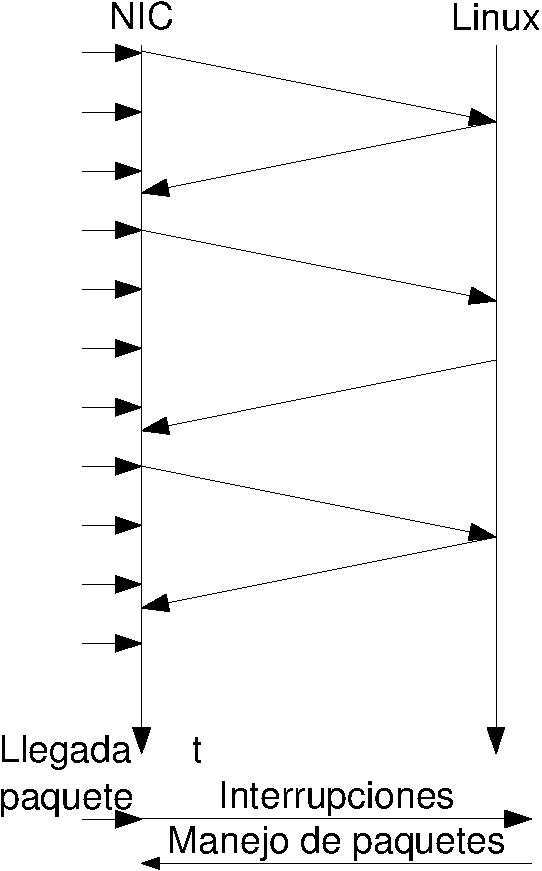
\includegraphics[width=0.30\textwidth]{CapituloPF_RING/Figuras/PollNIC-crop}}%
%
\caption{Comparativa entre los diferentes métodos de notificación de nuevos paquetes}
\end{figure}
%

\subsection{Obtención del paquete por parte del kernel}
Una interrupción debe ser rápida, esto es, en una interrupción no podemos realizar tareas que no sean estrictamente 
necesarias, por las mismas razones que las señales en espacio de usuario. Por ello, la interrupción provoca que se 
planee una tarea con el fin de recoger el paquete.

A partir de ese momento, sólo cuando el planeador decida que el sistema está libre, se recogerá el / los paquetes 
usando \texttt{packet\_rcv}, y se pasará a la pila de red de Linux.

En la pila, el paquete pasará por diversos sistemas, como la parte de filtrado 
\emph{\gls{netfilter}}\index{Netfilter} para, finalmente, ser recibido por un puerto o \emph{\gls{socket}} llegar a 
estar listo para la recogida por parte del espacio de usuario \cite{p206}.

\subsection{Obtención del paquete por parte del espacio de usuario}
La recepción de paquetes en el espacio de usuario se realiza mediante la librería \emph{\gls{libpcap}}\index{libpcap}.
Para ello, \emph{\gls{libpcap}} genera un \emph{\gls{socket}} que es abstraído por un descriptor de fichero. Si 
aplicamos la llamada al sistema \texttt{select} o \texttt{poll}, podemos saber si el socket dispone de datos para ser 
leídos, y leerlos en ese caso con la llamada \texttt{recvfrom}.

Un ejemplo de este tipo de lecturas podemos verlo en en \lstlistingname{}\ref{code:lecturaRawSocket}. En él, vemos la 
creación del socket con \texttt{socket}, la consulta de disponibilidad con \texttt{poll} y la recepción de los datos 
con \texttt{recvfrom}.

\begin{lstlisting}[language=C++,caption={Lectura desde un socket crudo}, 
breaklines=true, label=code:lecturaRawSocket,numbers=left,float=htbp]
#include<stdio.h>
#include<string.h>

#include<net/ethernet.h>
#include<sys/socket.h>
#include<arpa/inet.h>
#include<sys/ioctl.h>
#include<sys/types.h>
 
void ProcessPacket(char* , int);
 
int main(){
    size_t saddr_size, data_size;
    struct sockaddr saddr;
         
    char buffer[65536];
   
    int sock_raw = socket(AF_PACKET, SOCK_RAW, htons(ETH_P_ALL));
    setsockopt(sock_raw, SOL_SOCKET, SO_BINDTODEVICE, "eth0", 
                                               strlen("eth0")+1);
     
    if(sock_raw < 0){
        perror("Socket Error");
        return 1;
    }
    while(1){
        struct pollfd fds = { fd: sock_raw, events: POLLIN};
        const int poll_rc = poll(&fsd, 1, 1000);
        if(poll_rc == 0){
            if(poll_rc <= 0)
                perror("Poll error");
            continue;
        }
        saddr_size = sizeof(saddr);
        //Receive a packet
        data_size = recvfrom(sock_raw, buffer, 65536, 0, &saddr, 
                                       (socklen_t*)&saddr_size);
        if(data_size < 0){
            printf("Recvfrom error , failed to get packets\n");
            return 1;
        }
        //Now process the packet
        ProcessPacket(buffer , data_size);
    }
    close(sock_raw);
    return 0;
}
\end{lstlisting}

Sin embargo, este procedimiento tiene un coste oculto. A la hora de leer los datos, estos son copiados desde la 
memoria del núcleo a un buffer en espacio de usuario. Esto es, por cada paquete, estamos perdiendo tiempo y ciclos de 
CPU en copiar un dato que sólo vamos a leer.

Si, por ejemplo, queremos leer paquetes de 150kb en un enlace saturado a una velocidad de 1Gbps, estamos realizando:
\begin{itemize}
 \item $\frac{1G}{150k} \approx 7000$ llamadas al sistema con \texttt{poll} y otras tantas con \texttt{recvfrom}.
 \item Copiando entre regiones de memoria RAM a 1Gbps.
\end{itemize}

\section{La alternativa: PF\_RING}\LABSEC{La alternativa: PF RING}


\endinput

\begin{Resumen}[Resumen de PF RING]


\subsection*{S1}

\end{Resumen}

